\documentclass[12pt, a4paper, twoside]{book}
\usepackage{import}
\subimport{../}{preamble}
\onehalfspacing
\begin{document}

\begin{singlespace}
\chapter{Electrochemical Fabrication of Spherical AuNP-Tipped AFM Probes}
\end{singlespace}

\AddToShipoutPictureBG*{ \AtPageUpperLeft{ \put(0,-260)
{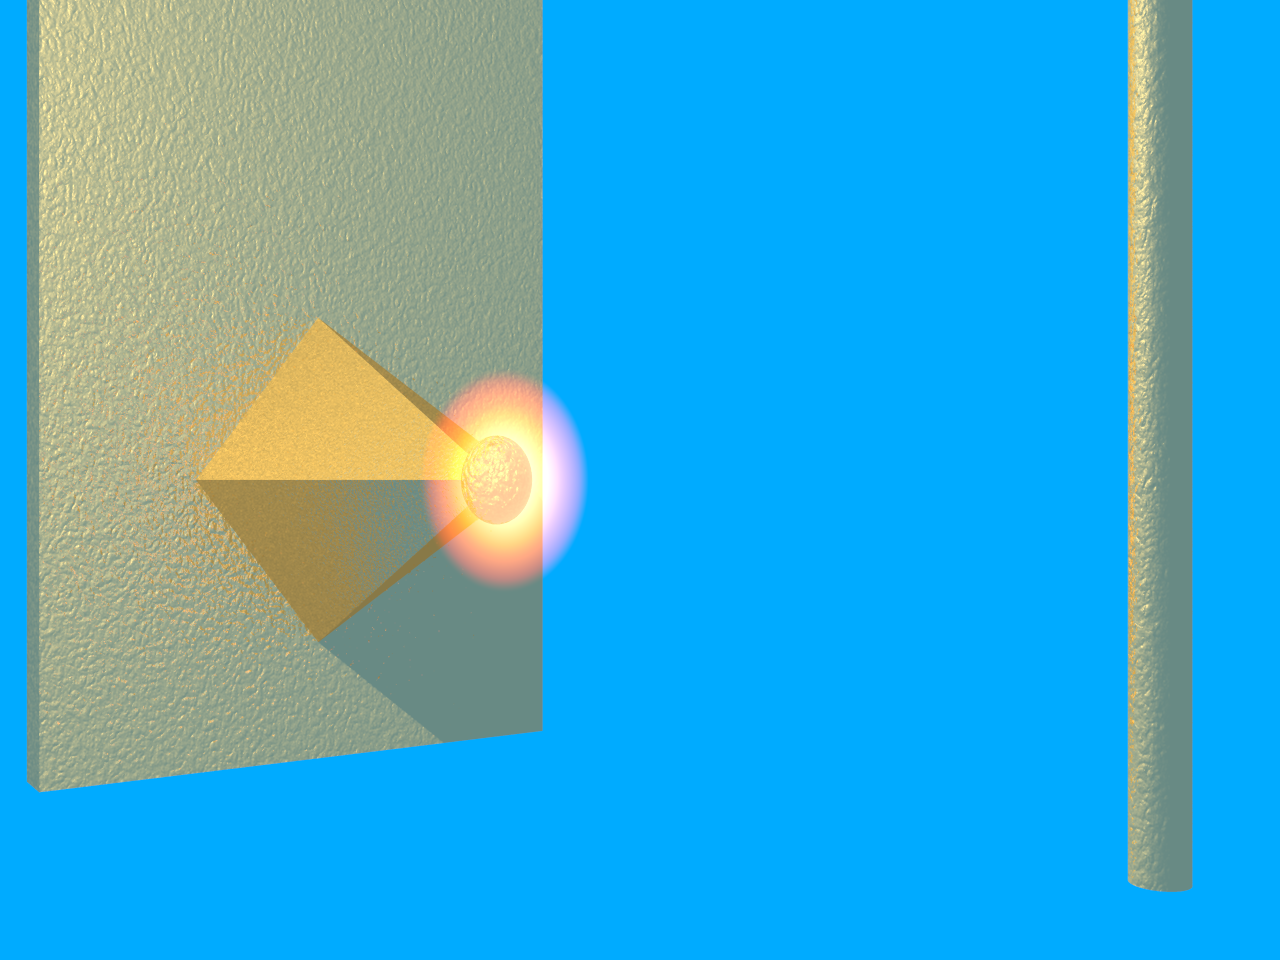
\includegraphics[width=\paperwidth, clip=true, trim=0 120 0 200]{data/chapter_cover.png}}
}}

As discussed in the previous chapter, nanostructuring a tip can create the necessary geometry and electromagnetic interfaces {\color{red}(increased electromagnetic density of states)} to support far-field antenna modes. This enables the coupling far-field light into plasmons and can improve the plasmonic performance of such tips. Consequently, this means that excited plasmons scatter into the far-field and are therefore observable. This is an important property when using tips to measure fundamental plasmonics. To this extent, one of the major aims of this project is to produce robust nanostructured, plasmonic tips. The spherical geometry is targeted for its simplicity.

Fabrication of spherical tips for plasmonics has been achieved by mounting single nanoparticles onto the apex of a tip. This concept has been reported numerous times over the last decade \cite{gan2007}, beginning with the use of fibres as mounting structures \cite{kalkbrenner2001, barsegova2002, sqalli2002, kawata2003} and progressing onto the use of scanning probe microscopy (SPM) tips \cite{umakoshi2012, hayazawa2012, park2012, okamoto2001, vakarelski2006}. Whilst mounting nanoparticles onto SPM tips is more difficult than with fibres the additional capabilities of the SPM tip have made such tips desirable. However, these tips typically require complicated assembly processes to precisely secure a single nanoparticle at the apex of the tip, greatly increasing their fabrication time and costs. More recent methods have attempted to address the complexity issue by directly depositing nanoparticles onto the apex by exploiting localised chemical reactions. However, these techniques have still been limited by cost or required specialist equipment \cite{sqalli2002, okamoto2001}, incompatible with SPM probes \cite{kharintsev2013, barsegova2002} or subject to limitations in nanoparticle growth, either in size \cite{cheng2013} or material \cite{umakoshi2012}.
%It remains a challenge to find a simple and efficient method for reliably producing spherical nanoparticle tips. Here we provide a simple and efficient method for reliably producing spherical nanoparticle tips using apex-selected electrochemical growth.
To date it is still a challenge to simply and efficiently produce spherically nanostructured tips. This chapter describes a simple method developed to produce spherical nanoparticle tips using apex-selected electrochemical growth.
The process of electrochemistry is first described followed by discussion of the original method of tip production and its limitations. A second method is then discussed, addressing the issues with the original method and showing how they can be circumvented but at the cost of production rate.

\subimport{./}{electrochemistry_theory}

Electrochemical deposition is highly suited to the tip geometry because of the large field enhancement localised at the sharp point. Due to the significantly reduced radius of curvature at the tip apex, the equipotential surface resulting from an applied voltage leads to compression of field lines in the region. This strongly increases the field amplitude at the tip apex and is known as the lightning rod effect. Under such conditions the rate of electrochemical reactions is significantly increased around the vicinity of the tip apex. By exploiting this localised field enhancement it is possible to grow a spherical nanoparticle directly onto the tip apex. Whilst use of the lightning rod effect for electrochemical growth has been used to grow dense forests of nanoparticles \cite{tian2006, yang2011} it has yet to be applied to the fabrication of single nanoparticles at the tips apex. A disadvantage of electrochemical deposition is that it is difficult to selectively grow nanoparticles on the tips. Here by using single-pulse high-field electrochemical growth, we selectively grow nanoparticles on the tip apex. Using this approach we demonstrate an efficient, high-throughput technique for reliably producing metallic spherical nanoparticle tips using only a simple electrochemical cell.

When aiming to grow a nanoparticle at the apex of an AFM tip the objective is not to obtain an even coating, hence well-documented techniques such as electroplating are not of use. Growth must be initially completely field dependent, taking advantage of the tip's lightning rod effect, but not over sufficient time that the smoothing of the apex curvature reduces the field and diverts growth around the resultant neck.

\subimport{./}{initial_fabrication}
\subimport{./}{modified_method}

%\subsection{Effect of Pre-Treatment}

%Without pre-treatment growth occurs somewhat as expected. Initial growth is at the apex which inevitably reduces the lightning rod effect by further rounding the tip. Growth occurs on all surfaces and the tip is more or less uniformly coated with a slightly thicker coating at the apex.

%\begin{figure}[h]
%\centering
%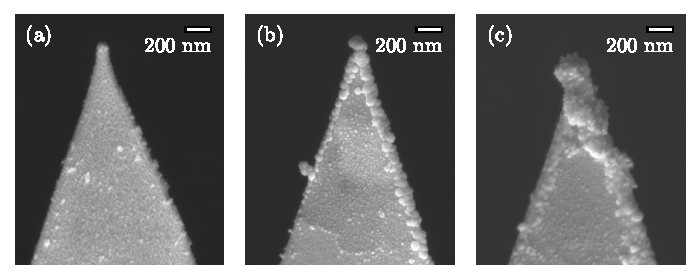
\includegraphics{figures/plasma_treatment_comparison}
%\caption{\label{fig:plasma_comparison} Plasma comparison}
%\end{figure}

%\section{Pre/Post-Treatment Options Required for Electrodeposited AuNP AFM Probes}

%Various chemical/physical processes are used during sample processing. The most effective strategy for successful AuNP tip fabrication requires \SI{20}{\minute} \ce{O2} plasma treatment prior to electrodeposition followed by submersion in piranha solution%
%\footnote{Piranha solution refers to a 3:1 mixture of \ce{H2SO4} and \ce{H2O2}, respectively. Small volumes (\SI{7}{ml}) are used to remove organic contaminants from surfaces with minimal heating but remain effective for less than \SI{1}{\hour}. Larger volumes ($\SI{\sim100}{ml}$) will reach temperatures of up to \SI{120}{\celsius}.}
%for \SI{1}{\hour} after SEMs have been taken.

\section{Conclusions}

By using electrochemical deposition, the simple fabrication of spherical metallic tips has been successfully demonstrated. Tips can be fabricated within a short period of time and with high throughput using pulsed electrochemical deposition and exploiting the sharp tip geometry to nucleate and grow a single nanoparticle at the apex. Though simple and cheap compared with many other techniques, control of growth morphology quality still presents issues.
Morphology control presents problems due to the many number of variables in the system, many of which were investigated to optimise and understand the deposition process. Despite significant efforts, the deposition process remains unreliable, though repeatable.
It has, however, succeeded in its original purpose of providing spherical Au tips for application to plasmonics.

\end{document}